\documentclass[tikz, border = 5pt]{standalone}
\usepackage{tikz}

\usetikzlibrary{arrows.meta}

\begin{document}

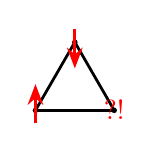
\begin{tikzpicture}[scale = 1.0]	

	% model Parameters
	\def \base{2}	% number of sites in base
	\def \a{1}	% lattice paramters

	% artistic parameters
	\def \lw{1pt}
	\def \arrowwidth{1pt}
	\def \arrowcolor{red}
	\def \fillcolor{black}
	\def \fillsize{1pt}


	% Create lattice points 
	\foreach \i in {1,...,\base}{
		\foreach \j in {1,...,\i}{
			\coordinate (P-\i-\j) at ({\a*(\i-0.5*\j)},{\a*\j*sqrt(3)/2});
		}
	}
	
	% Draw bubbles at lattice points, besides out outer most
	\foreach \i in {1,...,\base}{
		\foreach \j in {1,...,\i}{
			\fill[\fillcolor] (P-\i-\j) circle (\fillsize);
		}
	}

	% Draw nearest neighbour links
	\foreach \i in {1,...,\base}{
		\foreach \j in {1,...,\i}{
				
			% to right and top right:
			\ifnum \i < \base 
				\draw[line width = \lw] (P-\i-\j) -- (P-\the\numexpr\i+1\relax-\j);
				\draw[line width = \lw] (P-\i-\j) -- (P-\the\numexpr\i+1\relax-\the\numexpr\j+1\relax);
			\fi

			% to top left 
			\ifnum \j < \i
				\draw[line width = \lw] (P-\i-\j) -- (P-\i-\the\numexpr\j+1\relax);
			\fi	
		}
	}

	% draw symbols at corners of the triangle

	% upper corner

	
	% define arrow 
	% parmeters: center x, center y, length, rotation angle in degree (0 is positive x-direction)
	% optional parameters: color, line width


	\newcommand{\getpoint}[2]{%
    		\pgfmathsetmacro{\X}{\a*(#1-0.5*#2)}%
    		\pgfmathsetmacro{\Y}{\a*#2*sqrt(3)/2}%
	}

	\NewDocumentCommand{\drawarrow}{m m m m O{black} O{0.4pt}}{
	\getpoint{#1}{#2}
	\draw[-{Stealth}, line width = #6, draw = #5]({\X - #3*cos(#4)/3}, {\Y - #3*sin(#4)/3}) -- ({\X + 2*#3*cos(#4)/3}, {\Y + 2*#3*sin(#4)/3});
	}
	
	\drawarrow{1}{1}{0.5}{90}[\arrowcolor][\arrowwidth]
	\drawarrow{2}{2}{0.5}{270}[\arrowcolor][\arrowwidth]

	\getpoint{2}{1}
	\node at (\X, \Y) [red] {?!};

\end{tikzpicture}

\end{document}
